\chapter{Project Plan}\label{ch:project-plan}

\section{Methodology and Approach}
Project Plans

\subsection{Definitions}

\subsection{Overview}
The Assessments feature involves quizzes and polls, and aims at:

\begin{itemize}
    \item allowing submissions and grading to be performed on the same platform for convenience
    \item providing additional useful statistics as feedback to help improve the teachings of a course instructor and the learnings of a student enrolled in the course
    \item having an appealing, readable interface for both course instructors and students
\end{itemize}

The core features for quizzes include being able to:
\begin{itemize}
    \item create/remove/edit a question
    \item answer/edit an answer to a question
    \item choose between three types of questions to create:
    \begin{itemize}
    	\item multiple choice - select one answer only
    	\item short answer
    	\item checkboxes - select none, one or multiple answers
    \end{itemize}
    \item auto-save and manual save answers during quiz attempt
    \item timer that runs during quiz attempt
\end{itemize}

\begin{figure}[h!]
\centering
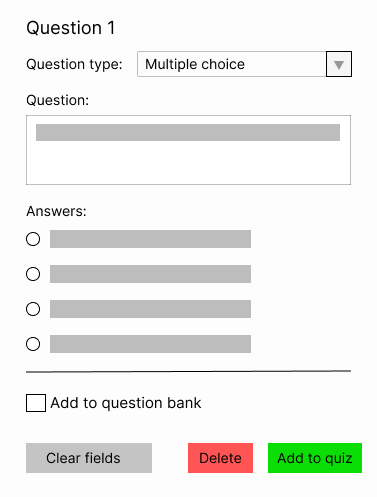
\includegraphics[scale=0.5]{quiz-creation}
\caption{Quiz creation (Instructor's view)}
\end{figure}

\begin{figure}[h!]
\centering
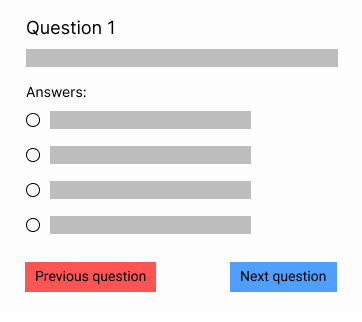
\includegraphics[scale=0.5]{quiz-usage}
\caption{Quiz usage (Student's view)}
\end{figure}

The core features for polls include being able to:
\begin{itemize}
	\item create/remove a poll
	\item create/remove/edit a poll option
	\item select poll options/s to vote and change your vote
	\item choose between two types of polls to create:
		\begin{itemize}
			\item restricted - can only vote for 1 option
			\item open - can vote for multiple options
		\end{itemize}
\end{itemize}


\subsection{Stakeholders}
\begin{itemize}
	\item Lecturer/course instructor
	\item Admins
	\item Students
\end{itemize}

\subsection{Functional Requirements}
The list of functional requirements' priority level will be determined using the MoSCoW method to clearly outline what needs to be implemented throughout the thesis and what the minimum viable product should have. 

The MoSCoW method splits requirements based on 4 categories:
\begin{itemize}
	\item Must Have
	\item Should Have
	\item Could Have
	\item Won't Have
\end{itemize}

A requirements survey was conducted and completed by me and other Thesis A students to gauge what was the priorities for each requirement. Below are the results for the Assessment features - quizzes and polls:

Must Have
\begin{itemize}
	\item Admins can create/remove quizzes/polls
	\item Admins can create/edit/remove questions in quizzes
	\item Admins can create different types of quiz questions (multiple-choice, short answer, checkboxes)
	\item Admins can set a timer for a quiz so that students must complete it within a set time
	\item Students can take quizzes/polls
	\item Admins can create/edit/remove options in polls
	\item Admins can create different types of polls (restricted to selecting 1 option, open to selecting multiple options)
\end{itemize}

Should Have
\begin{itemize}
	\item Admins can reuse questions from previous quizzes
	\item Students can view results of a quiz/poll
	\item Student, lecturers and admins can see how many students selected each answer for a question
\end{itemize}

Could Have
\begin{itemize}
	\item Drag and drop type questions
	\item "Connect the pairs" type questions
	\item Ability to add media (audio or video) into a question (as the question or as supplementary material)
	\item Students are displayed the topic or lecture the question derives from, if they answer it incorrectly
	\item Display an explanation of the correct answer if a student answers a question incorrectly
\end{itemize}

Won't Have
None

\subsection{Non-functional requirements}
\begin{itemize}
	\item Usability
	\item Re-usability
	\item Performance
	\item Extensibility
\end{itemize}


\section{System Architecture}
\subsection{Presentation Layer}
\subsection{Logic Layer}
\subsection{Data Layer}


\section{Timeline}
\subsection{Term 1 (Thesis A)}
Term 1 will mainly focus on literature research, outlining the main and potential features required to achieve the goals of this thesis. 

\begin{figure}[h!]
\centering
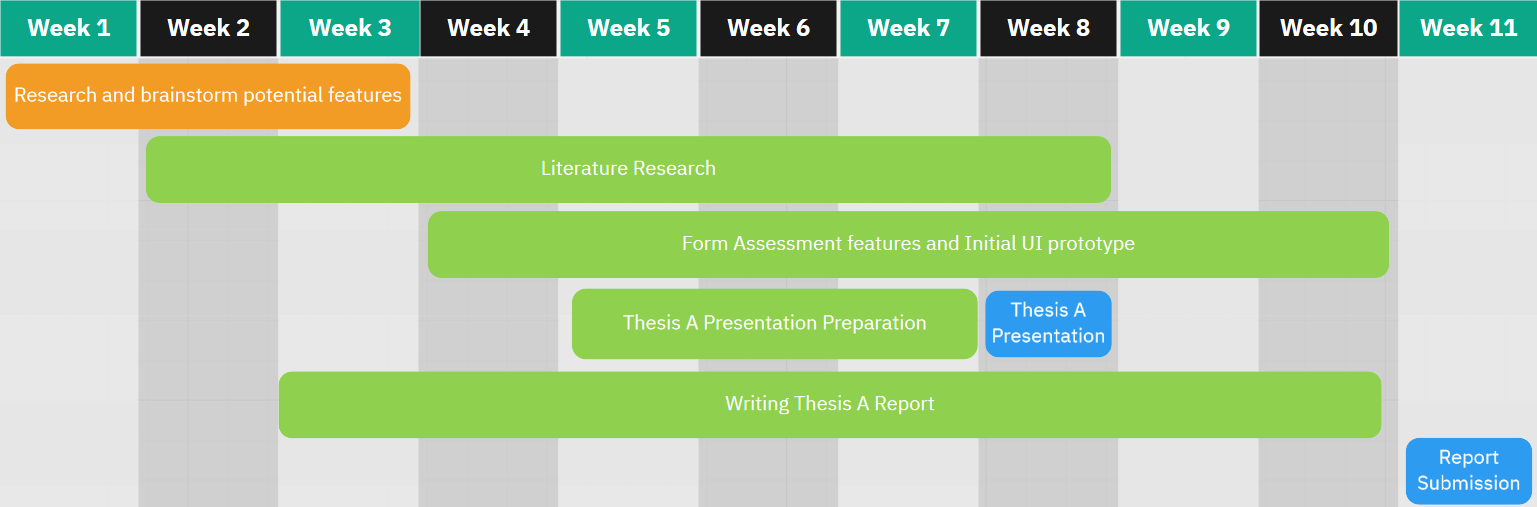
\includegraphics[scale=0.5]{term1-timeline}
\caption{Thesis A Timeline}
\end{figure}

\subsection{Term 2 (Thesis B)}
Term 2 will mainly focus on implementation of the core features and ensuring a good design overall before adding any extra features. 

\begin{figure}[h!]
\centering
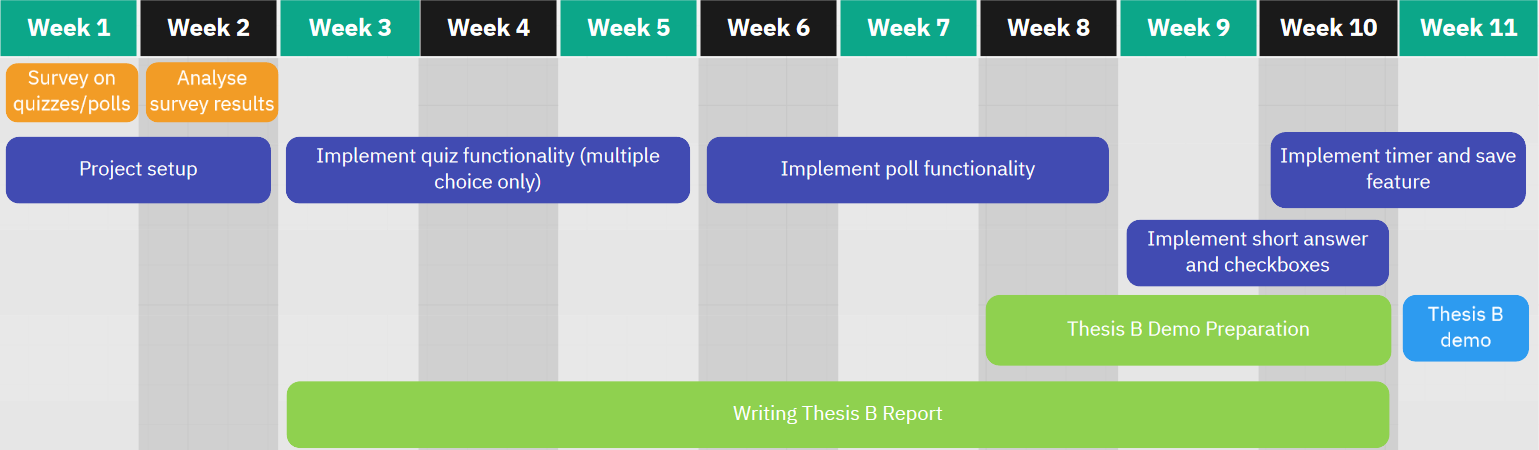
\includegraphics[scale=0.5]{term2-timeline}
\caption{Thesis B Timeline}
\end{figure}

\subsection{Term 3 (Thesis C)}
Term 3 will focus on improving the system based on feedback, implementing additional features and doing a final testing on the system to ensure it satisfies requirements. 

\begin{figure}[h!]
\centering
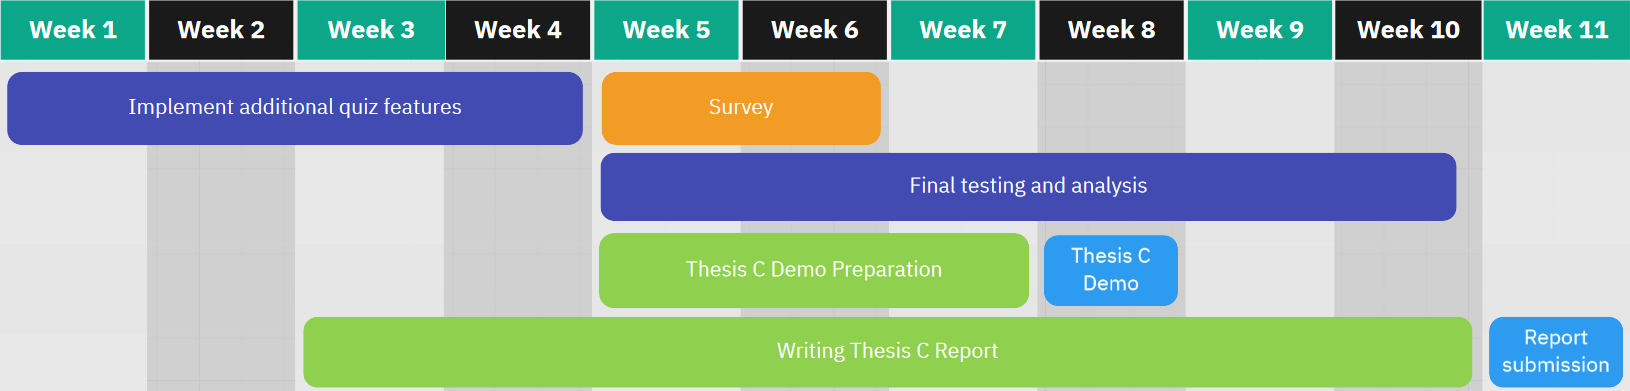
\includegraphics[scale=0.5]{term3-timeline}
\caption{Thesis C Timeline}
\end{figure}

\section{Required Training/Upskilling}
Training across multiple areas will be required in order to develop the Learning Management System:

\begin{itemize}
	\item Create technical diagrams using Miro (diagramming tool)
	\item Develop React skills
	\item Explore and experiment with graph visualisation libraries (to display statistics)
	\item Research SCORM and other standards used in learning management systems
\end{itemize}